\subsubsection{Purpose}
Both the mobile application and the web one provide the chance to any registered and logged user to view and update the personal profile information. The system is able to provide also information about the reservations and rides history as well as the respective payments.

Moreover the logged user is allowed to delete his/her account if the service is no longer needed.

\subsubsection{Scenario 1}
Anna has already carried out the registration process, but she does not like the password the system provided her because it is hard to remember. Therefore she decides to log in from her mobile phone and access the personal information area through the designated toolbar.

She taps \emph{"edit profile"} and the system allows her to edit profile information. Anna enters the old password in the designated field as well as the new one, that must be entered twice to avoid unwanted errors. Then Anna selects \emph{"Confirm"} and the system notifies her about the successful update.

\subsubsection{Scenario 2}
Flavio has recently renewed his identity card. In order to take the advantage of the \emph{PowerEnJoy} service, he must update his profile information. Flavio opens the browser, reaches the \emph{PowerEnJoy} home page and authenticates himself carrying out the login procedure. 

Then he access his personal information area and clicks \emph{"Edit Profile"}. He fills in the gap corresponding to the ID card number and, as soon as Flavio is ready, he clicks on the \emph{"Confirm"} button and the system confirms the ID card number has been successfully updated.

\subsubsection{Scenario 3}
Diana has carried out the subscription to \emph{PowerEnJoy} providing her credit card number. She creates a \emph{PayPal\textsuperscript{TM}} account and wants to use it as payment method whenever she rents a car. In order to do that, she logs in from her browser and accesses her personal information area.

Diana selects \emph{"Edit Profile"} and changes the payment method from credit card to \emph{PayPal\textsuperscript{TM}}. The system immediately asks for her \emph{PayPal\textsuperscript{TM}} credentials which will be used to perform payments automatically. She provides the information and confirms the change. The system informs her that the payment method has been successfully modified.

\subsubsection{Scenario 4}
Emma wants to delete her \emph{PowerEnJoy} account because she does not need the service anymore. She logs in from her mobile phone and enters her personal information area. She selects \emph{"Edit Profile"}, taps \emph{"Delete Account"} and confirms her choice twice. The system removes immediately all Emma's information from the database. From now on she needs a new account in order to access the system again.

\subsubsection{Use-case}
The overall profile management use-case diagram is shown in Figure \ref{man_profile_uc}. \\
The use-case of view profile procedure is analyzed in Table \ref{view_profile_uc}. \\
The use-case of modify profile procedure is analyzed in Table \ref{modify_profile_uc}. \\
The use-case of delete profile procedure is analyzed in Table \ref{delete_profile_uc}.

\subsubsection{Functional requirements}
\begin{enumerate}
\item The system allows logged user to view his/her profile. When the user enters his/her personal information area, the system must display:
	\begin{itemize}
	\item all the user's personal information that has been entered during the registration process;
	\item the rides and reservations history;
	\item the payments history.
	\end{itemize}
\item The system allows logged user to modify his/her personal information as needed:
	\begin{itemize}
	\item the system allows to change any information except e-mail address and authentication method related ones when the user selects \emph{"Edit Profile"};
	\item the system asks the user to enter the old password and two times the new one whenever he/she needs to change it;
	\item the system allows the user to change the password if and only if the old one has been entered correctly;
	\item the system must not allow the user to change the password if the new one has not been entered twice;
	\item the system makes the change permanent as soon as the user clicks the \emph{"Confirm"} button;
	\item the system allows the user to abort the profile editing at any time.
	\end{itemize}
\item The system allows the user to delete his/her account:
	\begin{itemize}
	\item the system asks for a confirmation twice whenever the user wants to delete his/her account;
	\item the system completely destroys the user's personal information and removes his/her account from the database.
	\end{itemize}
\end{enumerate}

\begin{figure}[H]
\begin{center}
		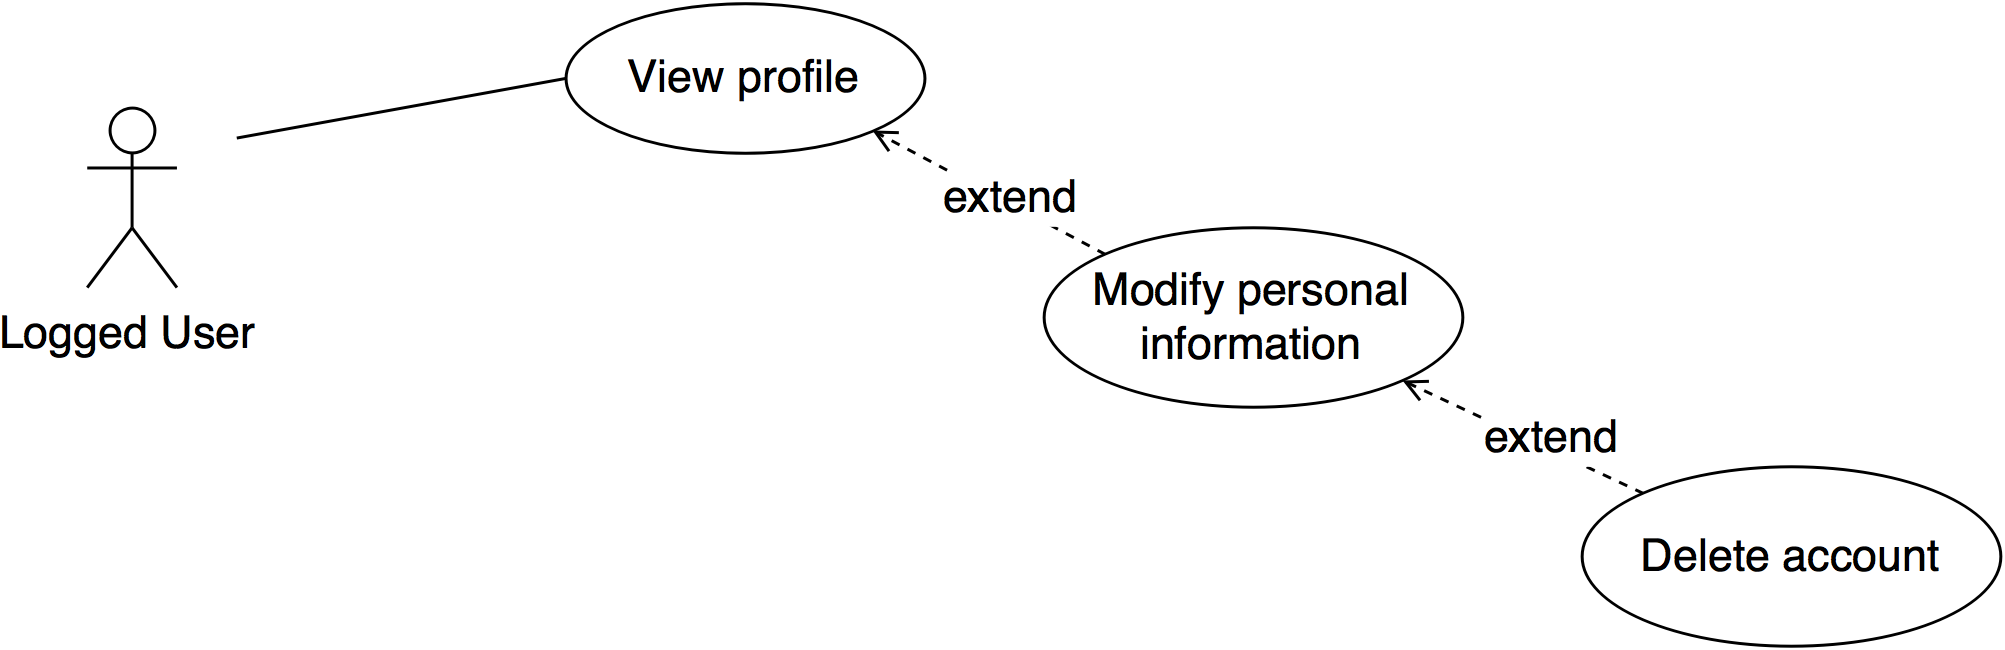
\includegraphics[width=\textwidth]{./specific_requirements/features/diagrams/man_profile_uc.png}
		\caption{Profile management use-case diagram.}
		\label{man_profile_uc}
\end{center}
\end{figure}

\begin{table}[H]
\begin{center}
\begin{tabular}{p{0.3\textwidth} | p{0.7\textwidth}}
\hline
Actor & Logged user\\
\hline
Goal & Goal 2\\
\hline
Input Condition & The user is already authenticated and wants his/her profile information to be displayed.\\
\hline
Event Flow & 
\begin{enumerate}
\item The user enters his/her personal information area.
\item The system loads the page.
\end{enumerate} \\
\hline
Output Condition & The system lets the user check his/her profile, the reservations and rides history as well as the completed payments.\\
\hline
Exception & 
None.\\
\hline
\end{tabular}
\end{center}
\caption{Profile visualization use-case.}
\label{view_profile_uc}
\end{table}

\begin{table}[H]
\begin{center}
\begin{tabular}{p{0.3\textwidth} | p{0.7\textwidth}}
\hline
Actor & Logged user\\
\hline
Goal & Goal 2\\
\hline
Input Condition & The user is already authenticated and wants to edit his/her profile information.\\
\hline
Event Flow & 
\begin{enumerate}
\item The user enters his/her personal information area;
\item The user selects \emph{"Edit Profile"};
\item The system loads the \emph{"Edit Profile"} page;
\item The user enters the new information;
\item The user confirms the desired changes.
\end{enumerate} \\
\hline
Output Condition & The system updates the user's personal information.\\
\hline
Exception & Every time the user does not satisfy one of the requirements listed as number 2, the system simply ignores the modification and reloads the \emph{"Edit Profile"} page.\\
\hline
\end{tabular}
\end{center}
\caption{Modify profile use-case.}
\label{modify_profile_uc}
\end{table}

\begin{table}[H]
\begin{center}
\begin{tabular}{p{0.3\textwidth} | p{0.7\textwidth}}
\hline
Actor & Logged user\\
\hline
Goal & Goal 2\\
\hline
Input Condition & The user is already authenticated and wants to delete completely his/her profile.\\
\hline
Event Flow & 
\begin{enumerate}
\item The user enters his/her personal information area;
\item The user selects \emph{"Edit Profile"};
\item The system loads the \emph{"Edit Profile"} page;
\item The user selects \emph{"Delete Account"};
\item The system asks to confirm and the user confirms;
\item The system asks again to confirm and the user agrees;
\end{enumerate} \\
\hline
Output Condition & The system deletes the user's account.\\
\hline
Exception & If the user decides not to confirm twice, the deletion process is aborted and the \emph{"Edit Profile"} page is reloaded.\\
\hline
\end{tabular}
\end{center}
\caption{Delete profile use-case.}
\label{delete_profile_uc}
\end{table}